\begin{center}
    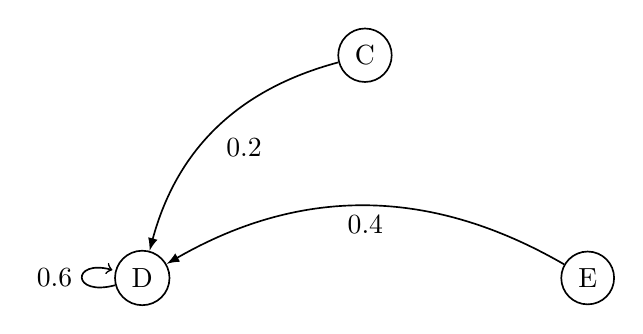
\begin{tikzpicture}[-latex, auto, node distance={4cm}, semithick, main/.style = {draw, circle}]
        \node[main] (C) {C};
        \node[main, below left of = C] (D) {D};
        \node[main, below right of = C] (E) {E};
        \path (C) edge[bend right] node{0.2} (D);
        \path (D) edge[loop left] node{0.6} (D);
        \path (E) edge[bend right] node{0.4} (D);
    \end{tikzpicture}
\end{center}